\documentclass[11pt]{article}
\usepackage[utf8]{inputenc}
\usepackage[T1]{fontenc}
\usepackage{lmodern}
\usepackage{amsmath,amssymb}
\usepackage{tikz}
\usepackage[margin=2.5cm]{geometry}
\setlength{\parindent}{0pt}
\DeclareMathOperator{\rect}{rect}

\begin{document}

% --- Fonction rect ---
\[
\rect(t) =
\vcenter{\hbox{
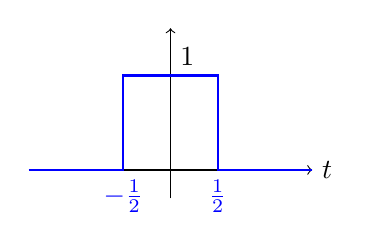
\begin{tikzpicture}[scale=1.2]
  \draw[->] (-1.5,0) -- (1.5,0) node[right] {$t$};
  \draw[->] (0,-0.3) -- (0,1.5);
  \draw[blue, thick] (-1.5,0) -- (-0.5,0) -- (-0.5,1) -- (0.5,1) -- (0.5,0) -- (1.5,0);
  \node[blue, below] at (-0.5,0) {$-\tfrac12$};
  \node[blue, below] at (0.5,0) {$\tfrac12$};
  \node[above right] at (0,1) {$1$};
\end{tikzpicture}}}
\]

\begin{align*}
& w(t) = \delta(t+8) + \delta(t+4) + \delta(t) + \delta(t-4) + \delta(t-8) \\
& \text{or } \delta(t-a) * h(t) = h(t-a) \\
& \Rightarrow f(t) = \sum_{k=-2}^{2} \rect(t - 4k) =
\vcenter{\hbox{
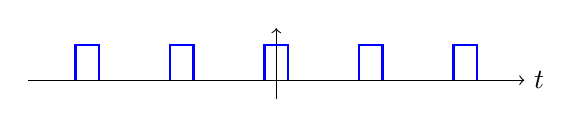
\begin{tikzpicture}[scale=0.3]
  \draw[->] (-10.5,0) -- (10.5,0) node[right] {$t$};
  \draw[->] (0,-0.8) -- (0,2.2);
  \foreach \c in {-8,-4,0,4,8} {
    \draw[blue, thick] (\c-0.5,0) -- (\c-0.5,1.5) -- (\c+0.5,1.5) -- (\c+0.5,0);
  }
\end{tikzpicture}}}
\end{align*}

3) Intercorrélation $C_{xy}$ entre $f$ et $\rect$\ldots

\medskip
\noindent\rule{\linewidth}{0.4pt}

\[
x(t) = e^{-t} u(t) \qquad\qquad h(t) = e^{-2t} u(t)
\]

\begin{align*}
y(t) &= \int_{-\infty}^{+\infty} u(\tau)\, e^{-\tau}\, e^{-2(t-\tau)}\, u(t-\tau)\, d\tau \\[4pt]
y &= \int_0^t e^{-\tau} e^{-2(t-\tau)}\, d\tau
   = \int_0^t e^{-2t+\tau}\, d\tau
   = \int_0^t e^{-2t} e^{\tau}\, d\tau \\[4pt]
y &= \Big[ e^{-2t} e^{\tau} \Big]_0^t = e^{-2t} e^{t} - e^{-2t} = e^{-t} - e^{-2t}
\end{align*}

\noindent\rule{\linewidth}{0.4pt}

\[
\begin{array}{lcl}
x^2 = 2^1 & \qquad\qquad & 9k^2 = 2^1 \\[10pt]
\dfrac{x}{3} = k & & x = 3k
\end{array}
\]

\end{document}
